\documentclass[conference]{IEEEtran}
\usepackage[dvips]{graphicx}
\graphicspath{{figs/}}
%\DeclareGraphicsExtensions{.eps}
\usepackage[cmex10]{amsmath}
%\interdisplaylinepenalty=2500
%\usepackage[tight,footnotesize]{subfigure}
%\usepackage[caption=false]{caption}
%\usepackage[font=footnotesize]{subfig}
%\usepackage[caption=false,font=footnotesize]{subfig}
%\usepackage{fixltx2e}
%\usepackage{stfloats}
\usepackage{url}
\hyphenation{op-tical net-works semi-conduc-tor}

\usepackage{multirow}
\usepackage{array}
\usepackage{footnote}

\widowpenalty=10000
\clubpenalty=10000

\begin{document}
\title{On the Design and Implementation of Secure, Private Overlays in
Constrained Environments}

\author{\IEEEauthorblockN{David Isaac Wolinsky and Renato Figueiredo} 
\IEEEauthorblockA{Advanced Computing Information Systems Lab\\
University of Florida}
}

\maketitle

\begin{abstract}
Using P2P overlays in distributed applications can significantly reduce the
cost for maintenance by their automated configuration, maintenance, and
optimization features.  Widespread adoption of P2P systems for home and small
business purposes has been limited to read-only data services such as data
transfer and streaming purposes in large part due to security concerns and
difficulty bootstrapping in constrained environments.  The requirements for
a P2P system in this context are structure, NAT traversal, point-to-point overlay
security, and a distributed data store.  Using these mechanisms, we propose
a novel way of creating trusted overlays or overlays that are both secure and
private by uisng a public overlay to coordinate discovery, security, and NAT
traversal.  Peers use the public overlay's distributed data store to discover
each other and then use the public overlay to assist with NAT hole punching
and as a relays providing STUN and TURN NAT traversal techniques.  Security is
provided by a group web site available through either the Internet or the
public overlay.  The group acts as a Public Key Infrastructure (PKI) relying on
the use of a centrally managed web site providing an automated Certificate
Authority (CA).  To qualify our design, we investigate different usage models
and present a reference implementation providing a P2P VPN (Virtual Private
Network).  Additionally, we evaluate our contributions using both the P2P VPN
in a live environment as well as event-based simulated time.
\end{abstract}
\section{Introduction}
Structured P2P overlays are largely self-managing though there has been a slow
adoption rate outside the using them for discovery services in data distribution
services such as BitTorrent and eDonkey and only as an optimization as the
systems are still reliant on centralized systems.  General use of structured
P2P systems, especially in home and small businesses, has been limited in large
part due to the difficult nature of securing such systems with a sufficient level
of trust.  Much previous work in securing these systems has focused on using
decentralized techniques for free-to-join systems.  Though home and small
businesses may need a greater level of trust than what can be guaranteed by
anonymous contributors in free-to-join overlays but lack the resources for
bootstrapping private overlays due to constrained environments, such as when a
significant amount of or all peers are behind Network Address Translation
devices (NAT).

There are many different applications for P2P use in home and small business
including data storage, media sharing, chat, and system maintenance and
monitoring.  While there are applications in this realm, they fall into two
categories, pure P2P systems that rely on anonymous sources and distributed
systems that rely on a third party to provide discovery and management.  While
using a third party service may reduce delivery time and provide a desirable
level of trust, it may also have long term effects such as vendor lock-in,
which may result in lost data, down time, and scalability constraints, all of
which create significant headaches.

An example of a useful small business application is LogMeIn's~\cite{logmein}
software products LogMeIn Pro and Hamachi.  LogMeIn Pro allows users to remotely
manage and connect with their machines so long as they are willing to use
LogMeIn's software and infrastructure.  Hamachi allows users to establish
decentralized VPN links using centralized session management.  Both
applications assist in the remote maintenance and monitoring of computers
without requiring the user to implement the networking infrastructure provided
by LogMeIn.

Some examples of P2P applications in development are P2PSIP and P2Pns, rapidly
evolving applications that have significant usefulness for homes and small
businesses.  P2PSIP enables users to initiate visual and audio communication
decentrally, while a P2Pns allows users to deploy a decentralized naming
service.  Both applications allow users to contribute and benefit from all
members of the system without the regulation of a third party but lack the
ability to allow users to centrally secure and manage their own subset of the
systems.

Distributed data store applications like Dynamo~\cite{dynamo} and
BigTable~\cite{bigtable} have the ability to store data using a completely
decentralized system.  Though these systems are highly scalable and fault
tolerant, the software uses an untrusted overlay.  Therefore all instances
should be run in a secure environment, whether that be in a single institution
or across a largely distributed environment using a VPN.

In this paper, we present a design and implementation of a system that attempts
to balance the benefits of third party services with P2P infrastructures.
Our system relies on a completely open infrastructure using mechanisms that
reduce the maintenance and deployment burden that exist with decentralized
P2P systems without the loss of ownership due to use of third party systems.
The components of our system follow:
\begin{enumerate}
\setlength{\itemsep}{0pt}
\setlength{\parskip}{0pt}
\item an application layer security system similar to DTLS to provide secure
end-to-end (EtE) and point-to-point (PtP) in P2P overlays while transparently
handling security concerns of relay NAT traversal;
\item a group web interface providing an automated front-end handler for a 
Public Key Infrastructure (PKI) that allows users to create their own secure
systems relying on P2P overlays;
\item the bootstrapping of private P2P overlays using existing public overlays,
because applying the concepts in this paper to a public free-to-join pool
is non-trivial.
\end{enumerate}

Our approach provides an easy mechanism to create trusted overlays in
constrained environments using a publicly available untrusted overlay.  This
model allows developers to focus on the application not concerning themselves
with the security of the system.  This approach also has benefits for system
deployers, whereas insecure systems would require modifying the overlay software
to support security,  application level security, or the deployment of a
decentralized and scalable VPN in addition to the overlay software.  Most
importantly our model provides a clean abstraction, which should make porting
applications sufficiently easy.

The rest of this paper is organized as follows.  Section~\ref{structured_p2p}
provides background on our and related work with emphasis on P2P systems.
Section~\ref{contributions} describes our contributions.  In
Section~\ref{applications}, we present different usage models and present a
real system using the techniques described in this paper, the GroupVPN.  In
Section~\ref{evaluations}, we use both real and simulated systems to provide
further understanding of the approach.  We conclude the paper in in
Section~\ref{conclusions}.

\section{Background}
\label{background}
In this section, we begin by reviewing structured P2P overlays, followed by
constraints that make the creation of secure and private P2P overlays
difficult, wrapping up with related work.

\subsection{Structured P2P Systems}
\label{structured_p2p}
Structured P2P systems provide distributed look up services with guaranteed
search time in $O(\log N)$ to $O(\log_2 N)$ time, in contrast to unstructured
systems, which rely on global knowledge/broadcasts, or stochastic techniques
such as random walks~\cite{unstructured_v_structured}.  Some examples of
structured systems can be found in~\cite{pastry, chord, symphony, kademlia,
can}.  In general, structured systems are able to make these guarantees by
self-organizing a structured topology such as a 2D ring or a hypercube.

The node ID, drawn from a large address space, must be unique to each peer,
otherwise an address collision occurs which can prevent nodes from participating
in the overlay.  Furthermore, having the node IDs well distributed assist in
providing better scalability as many algorithms for selection of shortcuts
depend on having node IDs uniformly distributed across the entire address space.
A simple mechanism to ensure this is to have each node use a cryptographically
strong random number generator.  Another mechanism for distributing node IDs
involves the use of a trusted third party to generate node IDs and
cryptographically sign them~\cite{secure_routing}.

As with unstructured P2P systems, in order for an incoming node to connect with
the system it must know of at least one active participant.  A list of nodes
that are running on public addresses should be maintained and distributed with
the application, available through some out-of-band mechanism, or possibly using
multicast to find pools~\cite{pastry}.

Depending on the protocol, a node must be connected to either the closest
neighbor smaller, larger, or both.  Optimizations for fault tolerance suggest
that it should be between 2 to $\log(N)$ on both sides.  If a peer does not
know the address of its immediate predecessor or successor and a message
is routed through it destined for them, depending on the message type, it may
either be locally consumed or thrown away, never arriving at its appropriate
destination.  Thus having multiple peers on both sides assist in stabilizing
when the experiencing churn, particularly when peers leave without warning.

Overlay shortcuts enable efficient routing in ring-structured P2P systems.  The
different shortcut selection methods include: maintaining large tables without
using connections and only verifying usability when routing
messages~\cite{pastry, kademlia}, maintaining a connection with a peer every
set distance in the P2P address space~\cite{chord}, or using locations drawn
from a harmonic distribution in the node address space~\cite{symphony}.

Most structured P2P overlays support the storing of arbitrary information by
mapping it to specific node IDs in an overlay.  At a minimum, the data is stored
at the node ID either smaller or larger to the data's node ID and for fault
tolerance the data can be stored at other nodes nearby.  This sort of mapping
and data storage is called a distributed hash table (DHT) and is a typical
component of most structured P2P systems.

\subsection{Constraints in Structured P2P Systems}
\subsubsection{Communication Between Nodes}
There are two mechanisms for message passing in a P2P overlay, iterative or
recursive.  In iterative routing, a peer sending a packet will contact each
successive member in a path directly until it find the destination node.  At
which point, it sends the packet directly to the destinataion.  In recursive
routing, messages are sent through the overlay via forwarding from one peer to
the next until arriving at the destination.  Iterative routing can easily be
secured using socket based security concepts such as TLS~\cite{tls} and
DTLS~\cite{dtls}, because there is no distinction between PtP
and EtE communication.  Whereas in recursive routing, EtE
communication will be an application primitive and rendering TLS and DTLS not
easily applicable.

\subsubsection{Private and Secure Overlay Subsets}
Secured ETE does not increase the reliability of a structured
overlay.  In a free-to-join system, malicious peers can easily intercept packets
and throw them away or tamper with them rendering them useless.  To deal with
this issue, each overlay node participate in a specific, secure EtE session,
could maintain a routing table that contains a subset of those involved.  The
approach would then require that the overlay support what is effectively a
second overlay but without an abstraction.  Requiring that each node instance
maintain multiple routing algorithms, state machines to handle fault tolerance,
and a mechanism for using a distributed data store only for the entire pool and
this subset.

\subsubsection{NATs}
Another issue present in P2P systems is the handling of NATs.  In environments
where there are NATs, iterative routing can be significantly more difficult to
deploy, since each message sent may require multiple NAT traversals.  With an
added layer of security, iterative routing can easily be too expensive to
deploy.   Additionally, TURN or relay style NAT traversal presents issues
similar to EtE in recursive routing, where each individual may authenticate
itself with the relay, they will not ebe able to easily use TLS and DTLS to
verify each other.

\subsection{Related Works}
BitTorrent~\cite{bittorrent_security}, a P2P data sharing service,  supports
stream encryption between peers sharing files.  The purpose of BitTorrent
security is not to keep messages private but to obfuscate packets to prvent
prevent traffic shapping due packet sniffing, thus BitTorrent security uses a
weak stream cipher, RC4, and lacks peer authentication as symmetric keys are
exchanged through an unauthenticated Diffie-Hellman process.

Hamachi~\cite{hamachi} provides central group management and a security
infrastructure through a web interface.  Their security system has gone through
two revisions as documented in~\cite{hamachi_security}.  Initially peers learn
of each other through Hamachi's central system, which leads to the creation of
secure links.  In their original approach, they use a system similar to a Key
Distribution Center (KDC), which requires that all security sessions initiate
through Hamachi's central servers.  In the latest version, this model has been
retained but with the addition of an external PKI, which avoids the
man-in-the-middle attack but with has the additional cost of maintaining both
an external CA and certificate revocation list (CRL).  Hamachi also supports
STUN and TURN style NAT traversal though TURN, again, requires the use of
Hamachi's own relay servers.  Because Hamachi is closed, it disables users from
hosting their own infrastructures including session management and relay
servers.

Skype~\cite{skype} like P2PSIP allows for decentralized audio and video
communication, though unlike P2PSIP Skype is well established and has millions
of users and is also closed.  While Skype does not provide documentation
detailing the security of its system, researchers~\cite{skype_auth,
skype_overview} have discovered that Skype supports both EtE and PtP security.
Though similar to Hamachi, Skype uses a KDC and does not let users setup their
own systems.

The RobotCA~\cite{robotca} provides an automated approach for decentralized
PKI.  A RobotCAs receives request via e-mail, verifies that the sender's e-mail
address and embedded PGP key match, signs the request, and mails it back to the
sender.  RobotCAs are only as secure as the underlying e-mail infrastructure
and provide no guarantees about the person beyond their ownership of an e-mail
address.  A RobotCA does not provide features to limit the signing of
certificates nor does it provide user-friendly or intuitive mechanisms for
certificate revocation.

\cite{one_ring} proposes the use of a universal overlay as a discovery plane for
service overlay.  The argument is that as a participant of an overlay, you
must support all services provided by that overlay such as multicast, DHT,
or distributed search.  Our work has the same foundations as this proposal but
takes the idea further by using the universal overlay for NAT traversal;
the service overlays become limited access, private overlays; and we have
a prototype implementation, which is reflected in our well-defined design.

Distributed data store applications like~\cite{dynamo, bigtable} require that
all machines have symmetric connectivity additionally like~\cite{past} suggest
the use of a third party application to ensure trust amongst all overlay
participants.  This is an example use case that is explicitly targeted by our
system on the presumption that there are not sufficiently easy to use
decentralized VPN software applications~\cite{sc09, nsdi10} and even if there
were it is undesirable to have additional setup requirements.

While there has been much research~\cite{secure_routing} in securing overlays
through decentralized mechanisms that attempt to prevent a collusion known as
a sybil attack~\cite{sybil}, these mechanisms do not create private overlays.
While one approch is mentioned does provide a natural lead into such
environments which is the use of a pay to use service to mitigate the chances
of an overlay attack, whereby the pay to use service uses a CA to sign node
IDs.  The work does not describe how to efficiently implement such a system.
Other similar research attempts to create trusted systems~\cite{stone, tor} but
with anonymous members, though it could be reasonably argued these services are
not applicable to small or medium business, which would prefer to have a private
overlay.  None of the works discuss how to apply such models to constrained
systems.

\section{Bootstrapping Secure and Private Overlays}
\label{contributions}
In this section, we explain the individual components of our contribution.  We
begin by describing how apply a DTLS like protocol for EtE and PtP security in
P2P systems, which leads to a discussion of using a group web interface to
provide a user-friendly PKI, and conlude with our approach to bootstrapping
private and secure overlays in constrained environments using public overlays.

\subsection{Secure Overlays}
\label{secure_overlays}
Securing EtE and PtP communication in overlays using iterative routing with
servers using static IP addresses can easily be done using TLS or DTLS with
certificates bound to the servers static IP address.  This approach does not
port well to systems that use recursive routing, TLS cannot easily be used
because overlay routing is traditionally done through datagrams not streams,
which would require overlays to implement a reliable stream to use TLS.  Where
as DTLS can be applied though it must support being used without a socket.  The
problem then becomes how to deal with identity.  In this section, we discuss how
to bind security protocols and a certificate model to an overlay system.

The key to our approach is abstracting the communication layer making EtE and
PtP traffic appear identical, thus all messages are datagrams that are sent
over abstracted senders and receivers, as illustrated in
Figure~\ref{fig:senders_receivers}.  This allows us to use secure tunnels over
these links with no application changes.

\begin{figure}[h]
\centering
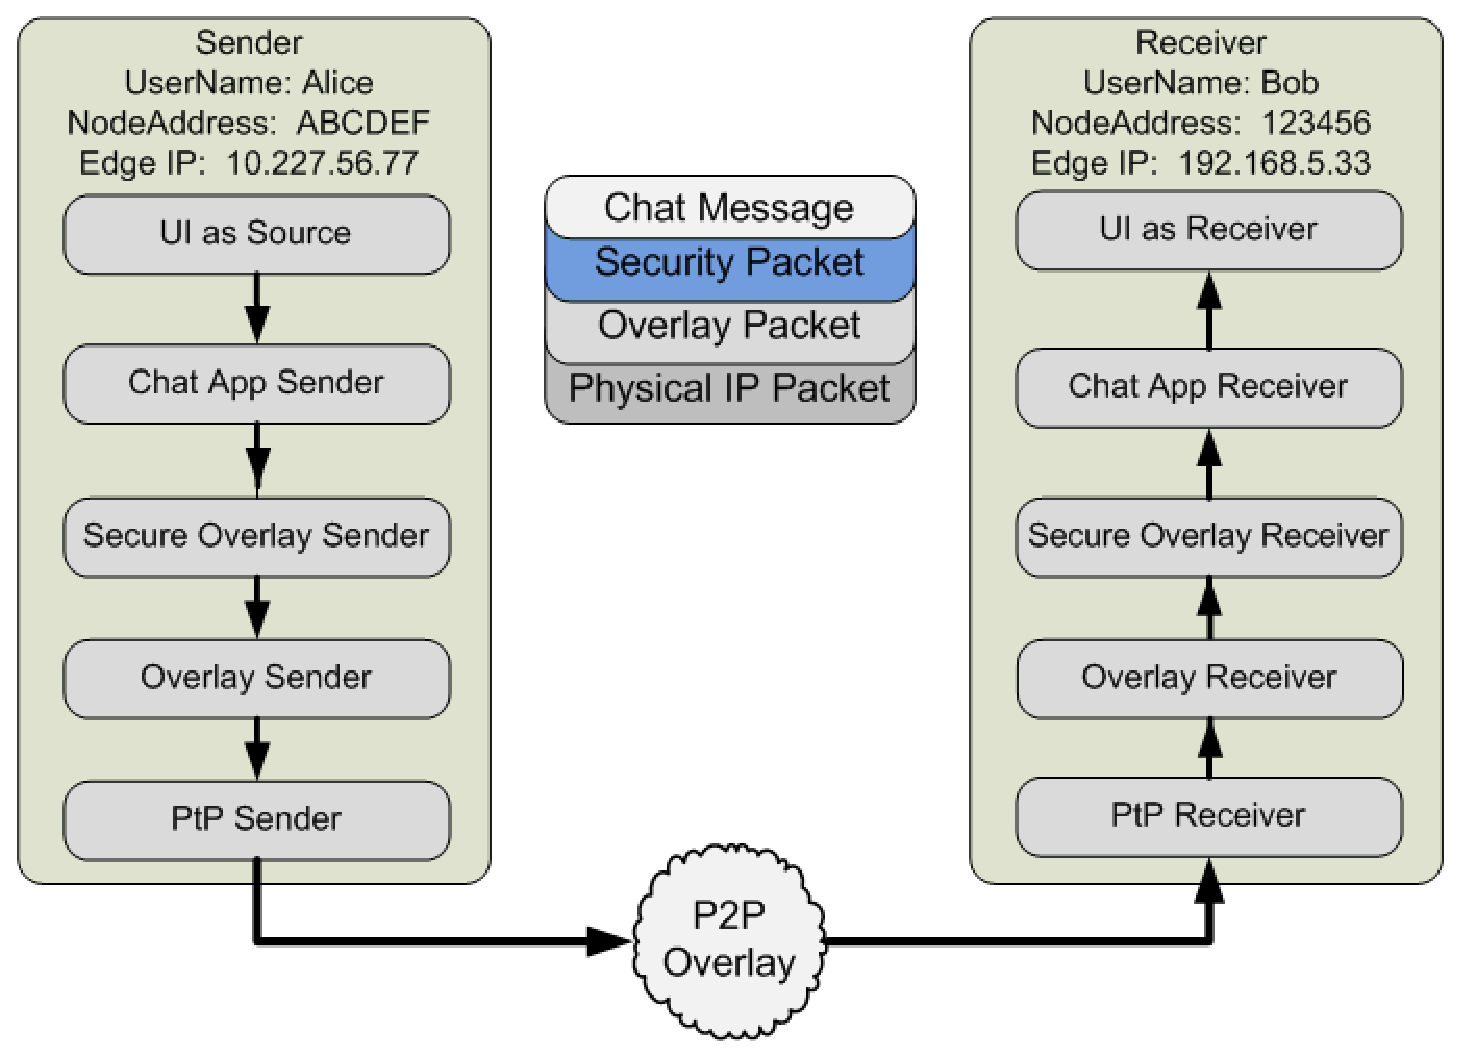
\includegraphics[width=3.25in]{secure_sender_stack_generic.png.eps}
\caption{An example of the abstraction of senders and receivers using a EtE 
secured chat application.  Each receiver and sender use the same abstracted
model and thus the chat application requires only high-level changes, such
as verifying the certificate used is Alice's and Bob's, to support security.}
\label{fig:senders_receivers}
\end{figure}

Exchanged certificates need a mechanism to verify authenticity.  Like an
Internet browser, this verification should happen automatically with no user
intervention.  Typically for TLS and DTLS certificates have the web sites
IP address or domain name as part of the certificate's common name field.  In
our system, we bind the certificate to each individual node ID.  That way,
a single certificate cannot be used for multiple peers in the overlay slowing
down potential sybil attacks.

\subsubsection{Forming the Connection}
In overlay systems, a peer's connection manager requests to make an outgoing
connection to another peer in the system.  This triggers the creation of a
UDP or TCP socket, which are wrapped in the abstracted sender and receiver
models.  The abstracted models arrive into the security handler, which
authenticates in both directions and create a secure session.  The session is
wrapped in the same abstracted model and presented to the overlay system as a
direct connection to the remote peer.  To keep the system abstract, the security
model and the wrapped sockets know nothing about the overlay, and so the overlay
should verify the certificate to ensure identity.

Because EtE communication is application specific and not run-time, it requires
a slightly different path.  For that purpose, we have a specific module that
allows an application to request a secure EtE sender but will deal with the
process of handling verification.  Once an application requests the sender, the
module passes a sender / receiver model to the security handler, like the PtP
process.  Once the security initialization has completed, the
resulting sender / receiver is verified automatically for proper identity.
If that succeeds, messages sent using the EtE sender will arrive at the remote
party, decrypted and authenticated by the security handler, and delivered to the
overlay application who will deliver to remote party's handler for such messages.
Creating one issue, since overlay application will be sending and receiving
unencrypted as well as encrypted EtE traffic, the handler must verify that the
packet was sent from a secure end point.  This assumes that an application using
an overlay has already implemented verification of node ID to some application
mapping.  For example, an application could be aware that node ID X maps to user
Y, therefore if a secure message coming from node ID Z says that it is user Y,
an application should throw the packet away.

\subsubsection{Datagram Constraints}
Since UDP is connectionless, applications that use it can easily be victims of
denial of service attacks.  This is because, packets sent to the receiver can
have a spoofed source address unless the outgoing gateway prevents this from
occurring.  Whereas with TCP, it would be signficantly harder to perform the
same attack unless performed as a man-in-the-middle.  To reduce the potential
of these spoofing attacks prior to establishing a secure connection, DTLS like
Photuris~\cite{photuris} uses a stateless cookie for each remote peer.  In
DTLS, the cookie is usually based upon the remote peers IP and the current
time.  In our model, which deals with abstracted systems, this approach will
not work.  Though because we are building on existing senders and receivers
that already have state, we can use the objects memory pointer or hash value
instead.

Since symmetric keys work on limited block size, they use modes of operation
to encrypt or decrypt large sets of blocks.  Because DTLS uses an unreliable
transfer mechanism, each message should be able to be decrypted without the use
of previous messages.  As suggested in the DTLS paper, we used cipher-block
chaning (CBC) with a new initialization vector (IV) for each message.  During
analysis, we discovered that generating a truly random IV was expensive but the
initialization of an additional CBC state machine was even more.  To reduce
these costs, the sender always uses the same CBC state machine and prepends
the last cipher-block to the beginning of the next message.  Upon reception,
a receiver compares the prepended message to a cache of CBC state machines
stored by the current state, if there is a match, then the CBC state machine
can be used, otherwise, if the packet is received out of order the receiver
can start a new CBC state machine to decrypt the packet.  Table~\ref{tab:cbc_issue}
compares the overhead with the default implementation and with our revised
version.

\begin{table}[h]
\setlength{\itemsep}{0pt}
\setlength{\parskip}{0pt}
\centering
\begin{tabular}[c]{|m{1.5cm}||m{3cm}|m{3cm}|} \hline
& Latency (ms) & Bandwidth (Mbit/s) \\ \hline\hline
DTLS CBC & 0 & 0 \\ \hline
Our CBC & 0 & 0 \\ \hline
\end{tabular}
\caption{CBC Issue -- In Progress.}
\label{tab:cbc_issue}
\end{table}

\subsection{Group Overlays}
\label{group_overlays}
To establish trusted links, we use the PKI model, where a centralized CA signs
all client certificates and clients can verify each other without CA interaction
by using the CA's public certificate.  However, setting up, deploying, and then
maintaining security credentials can easily become a non-negligible task,
especially for non-experts.  Most PKI-enabled systems require the use of
command-line utilities and setting up your own methods for securely
deploying certificates and policing users.  While this can be applied to an
overlay, our experience with real deployments indicates that usability is very
important, leading us to find a model with easy to user interfaces.
In this section, we present our solution, a partially automated PKI reliant on
a redistributable group based web interface.  Although this does not preclude
other methods of CA interaction, our experience has shown that it provides a
model that is satisfactory for many use cases.

\subsubsection{Joining the Group Overlay}
Membership of an overlay maps a set of users as a group, this led us to the
model of using a group infrastructure as a means to apply a PKI.  Using our
system, a user can host an individual or multiple groups per a web site.  The
creator of the group becomes the default administrator and users can request
access to the group.  Upon an administrator approving, users are able to
download configuration data containing overlay information and a shared key
used by the overlay application to communicate securely with the web interface.
The shared key uniquely identifies the user to the web site allowing the
application to securely send certificate requests.  By default, the web site
automatically signs all certificate requests, but the application and web site
support different models.  Two other models are 1) require the user to
submit a request and wait for an administrator to verify each request and 2)
set a maximum amount of automatic request signings and then require the 
administrator to reset the value upon using all of them.

As stated in Section~\ref{secure_overlays}, the certificate request is bound
to the applications node ID, which can be generated by the CA or the
application.  Additionally in the group system, the certificate also contains
the user who made the request and the group for which the certificate is valid.
Not only does this ensure that a single certificate can only be used for each
node instance, but it reduces the amount of state necessary to revoke a user
from a system.  Specifically, to revoke a user, the CA would only need to
provide a signed revocation notice containing the user's name and not every one
of the previously signed certificates.

Upon receiving a signed certificate, the overlay application can connect to the
overlay where all PtP traffic will be secured and, optionally, so can EtE
traffic.  It is imperative that any operations that involve the exchanging of
secret information, such as the shared secret, be performed over a secure
transport, such as HTTPS, which can be done with no user intervention.

\subsubsection{Handling User Revocation}
Unlike decentralized systems that use shared secrets, in which the creator of
the overlay becomes powerless to control malicious users, a PKI enables the
creator to effectively remove malicious users.  The methods that we have
incorporated include:  use of a user revocation list hosted on the group server,
DHT events requesting notification of peer removal from the group, and
broadcasting to the entire P2P system the revocation of the peer.

A user revocation list offers an out of band distribution mechanism that can
not easily tampered, whereas communication using the overlay can be hampered
by sybil attacks.  The revocation list is maintained on the website and updated
whenever an administrator removes a user or a user leaves the group,
additionally it is updated every 24 so that user can verify that the revocation
list is up to date.

Though because the user revocation list requires centralization, users should
not query it prior to every communication nor periodically during conversations.
As such, the use of the DHT and broadcast assist provide active notification of
user revocation.  The DHT method allows users to request notification if a peer
is revoked from the group.  The method for doing this is for the user to place
their node ID at the peer's revocation notification key.  Whereupon revocation,
the CA will query the key for its values and notify all the users of the
revocation.  Whereas the broacast mechanism notifies all active peers in the
overlay of the revocation.

When the group is securing PtP traffic, the DHT approach does not effectively
seal the rogue user from the system until all peers have updated the revocation
list.  Due to this issue, we do not employ this model in the group overlay.
Instead a broadcast will ensure that all peers in the system do know about
the revocation.  The strength of the DHT approach exists when using a public
free-to-join and an application secured by the group, as we did with a VPN in
~\cite{nsdi10}.

In Figure~\ref{fig:broadcast_revocation}, we present the cost of revoking a
peer in varying sized networks.  To evaluate the cost, we estimate that the
average size of a revocation is 300 bytes, which includes information such
as the user's name, the group, time of revocation, and a signature from the
CAs private key.  We then evaluate the bandwidth and latency cost using a
network modeler that reuses the same code base, i.e. routing tables and routing
algorithms, as our structured P2P overlay software.  For latency estimation,
we apply the MIT King data set~\cite{king_data}.

\begin{figure}[h]
\centering

\includegraphics[width=2.75in]{in_progress.eps}
\caption{Broadcast revocation.}
\label{fig:broadcast_revocation}
\end{figure}

Another approach would be to use the additional certificate revocation list
(CRL) used in most CA systems.  The advantage of a CRL and revoking individual
certificates is the ability to remove a subset of a user's node, particularly
useful in the case that the user was not malicious but that some of their nodes
had been tampered or hijacked.

\subsection{Private Overlays}
The main components involved in the starting and maintaining a private overlay
are 1) dissemination of the groups security credentials and its name, 2) 
connecting with and storing data in the public overlay, and 3) discovering and
connecting with peers in the private overlay.  1) is taken care of by the group
interface as described in Section~\ref{group_overlays}.  For 2), we presume the
usage of a structured overlay as described in Section~\ref{structured_p2p}.  In
this section, we discuss 3), the steps involved in creating and connecting to a
private overlay after the user has obtained group information and has connected
to a public overlay.

To connect with and create a private overlay, the application performs the
following steps:
\begin{enumerate}
\setlength{\itemsep}{0pt}
\setlength{\parskip}{0pt}
\item connects with the public overlay
\item stores its node ID in the public overlay's DHT at the private group's key
\item queries the public overlay's DHT at the private group's key
\item start an instance of the private overlay with the well-known end points
being those of the node IDs retrieved from the DHT
\item upon forming a link with a member in the private overlay, the node follows
the general approach for connecting to overlays
\end{enumerate}

The node should maintain membership in the public overlay when connected with
the private overlay.  For two reasons, one so that other peers can discover the
node while following the same set of steps and two for NAT traversal purposes
discussed in the next paragraph.  Because the public overlay and its DHT
provides a means for discovery, nodes must maintain there node ID in the public
key's DHT.  A data inserter must constantly update the lease for the data
object, otherwise the data will be removed.  This is because DHTs are
implemented as leasing systems, whereby data objects are inserted with a time
to live and removed upon expiration.

During the formation of the private overlay, peers may find that they are
unable to form direct connections with members of the private overlay.  For
this, we have two solutions, 1) to use TURN NAT traveral as discussed
in~\cite{nsdi10} and 2) use the public overlay as an extra routing massive TURN
infrastructure.  The TURN NAT traversal technique has both peers connect with
each others near neighbors in order to form a 2-hop connection with each other.
The 2-hop route can either be enforced through a static route or through EtE
greedy routing.  Due to the abstractions in the system, the public overlay can
be treated as another mechanism to create PtP links, thus while packets may use
EtE routing on the public overlay the private overlay nodes treat it as a PtP
connection thus all communication is secured.  This approach can be further
enhanced by allowing the private overlay to apply the TURN NAT traversal
technique to the public overlay.  To do this, the private overlay must be
capable of requesting a direct connection between the its node and the remote
peer in the public overlay.  This would trigger the eventual creation of a 2-hop
relay connection as presented in Figure~\ref{fig:overlay_relay}.

\begin{figure}[h]
\centering
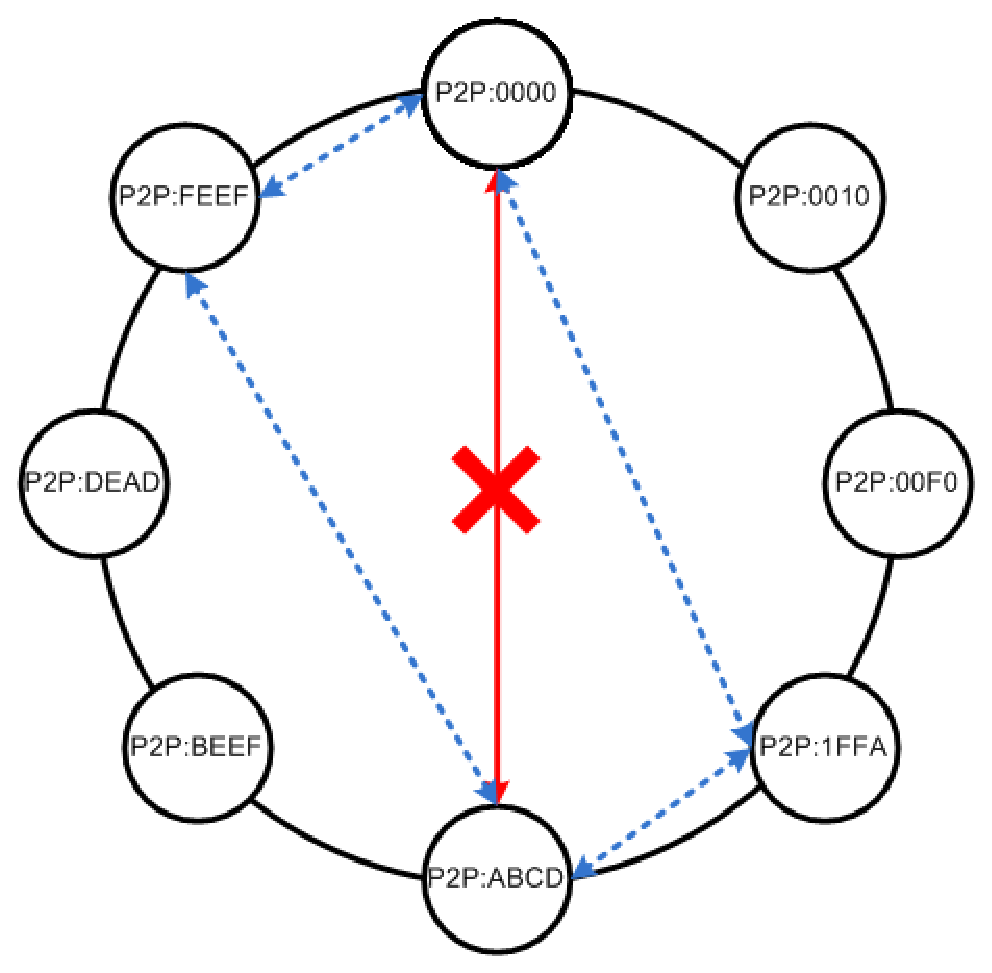
\includegraphics[width=2.75in]{relay.png.eps}
\caption{Creating relays across the node address space, when direct
connectivity is not possible.  Two members, 0000 and ABCD,  desire a direct
connection but are unable to directly connect, perhaps due to NATs or firewalls.
They exchange neighbor information through the overlay and connect to one of
each other's neighbors, creating an overlap.  The overlap then becomes a
relay path (represented by dashed lines), improving performance over routing
across the entire overlay.}
\label{fig:overlay_relay}
\end{figure}

Another concern we address is the cost of having to maintain additional
connections for each additional private overlay.  For this, we created a notion
called paths, which multiplexes a single UDP or TCP socket to support multiple
overlay nodes.  This model is supported because of the abstraction done on
senders and receivers.  Thus a UDP or TCP connection can be easily wrapped 
inside an abitrary packet, in this case, a pathing connection.  Upon sending
a packet, the message is prepended with path information.  When the remote side
receives a packet, it parses and removes this pathing information and relays it
to the appropriate receiver, i.e., overlay node.  To validate this apparoch, we
present the tradeoffs of this approach in Figure~\ref{fig:pathing_eval}, which
presents the network latency verse memory costs for varying sized pathing systems.

\begin{figure}[h]
\centering

\includegraphics[width=2.75in]{in_progress.eps}
\caption{Pathing evalution.}
\label{fig:pathing_eval}
\end{figure}

When overlays are small and have significant churn, it is easy for data stored
in the overlay to be easily lost.  This can be improved by implementing
MapReduce~\cite{mapreduce} in the overlay.  In this model, each peer acts as a
storage point for all data critical to itself.  If another peer cannot
successfully find data stored at a specific key in the overlay, it can use
MapReduce to broadcast the request to the entire overlay in an attempt to find
the result.  We present a comparison of the time and network cost for both
approaches in Figure~\ref{fig:mapreduce_cost}.

\begin{figure}[h]
\centering

\includegraphics[width=2.75in]{in_progress.eps}
\caption{MapReduce cost.}
\label{fig:mapreduce_cost}
\end{figure}

\section{Applications}
\label{applications}
\subsection{Instant Messaging}
\subsection{Data Sharing}
\subsection{P2P VPNs}
\section{Evaluation}
\label{evaluations}
In this section, we describe our prototype implementation of a secure, private
overlay followed by evaluation to quantify network, memory, and CPU overheads.
\subsection{Our Implementation -- Brunet}
Our implementation is based upon Brunet~\cite{brunet}, which is a P2P system
based upon the concepts introduced by Symphony~\cite{symphony}.  Thus it is a
one-dimenesional ring, where peers connect with up to the four peers closest
to themselves in both directions in the node ID space.  Shortcuts are based
upon a harmonic distribution and the use of of proximity~\cite{hpdc08_0}.  The
system supports both STUN based NAT traversal as well as a TURN-like system
~\cite{nsdi10}.  The system uses a DHT as a distributed data store using a
replication algorithm that spreads a single key, value pair throughout the ring
as described in~\cite{pcgrid07}.  Additionally, the overlay has support for
autonomic~\cite{wow} and manual creation of single-hop connections and double-hop
through relaying when NATs prevent direct connections.  Furthermore, we have
developed a P2P VPN on top of this stack, which has been used for over three
years to support a ad hoc distributed grid~\cite{archer, gridappliance}.
\subsection{Exploring Overheads}
\section{Conclusion}
\label{conclusions}
In this paper, we presented a novel architecture for deploying secure, private
overlays in constrained environments through the use of a public overlay.
The public overlay at a minimum need only to support a distributed data store,
like a DHT, so that peers of the private system can rendezvous with each other.
For constrained environments, we used NAT traversal techniques like STUN and
TURN with both private and public overlays supporting the relaying of packets.
We evaluated the use of DTLS in our system and presented an improved CBC
mode of operation for use in datagram systems that significantly speeded up our
implementation.  To deal with excessive amounts of sockets, we introduced the
notion of pathing, which showed that system resource consumption can be reduced
with negligible effect on network performance.  Most importantly, we presented
how a group infrastructure can be used as a user-friendly and intuitive
mechanism to create and maintain trusted overlays.  For future work, we envision
applying this approach to social networks and to establish multicast groups as
done in~\cite{can}.
%\section*{Acknowledgment}

\bibliographystyle{IEEEtran}
\bibliography{icdcs10}
\suppressfloats

\end{document}
